\documentclass[xcolor={usenames,dvipsnames}]{beamer}

\usepackage[utf8x]{inputenc}

\definecolor{solarbg}{HTML}{FDF6E3}

\usepackage{minted}
\newminted{c}{frame=single}
\usemintedstyle{solarized}

\usetheme{Antibes}
\usecolortheme[named=Bittersweet]{structure}

\title[Glift: Generic, Efficient, Random-Access GPU Data Structures]%
      {Glift:\\ Generic, Efficient, Random-Access GPU Data Structures}
\author{Jean Niklas L'orange}
\institute{\texttt{jeannikl@hypirion.com}}
\date{October 15, 2013}

\begin{document}

\begin{frame}
  \titlepage
\end{frame}

\section{What and why?}
\begin{frame}
  \frametitle{What is this paper about? What is Glift?}

  This paper is about a data-parallel programming abstraction. The abstraction
  enables GPU programmers to write high-level, efficient random-access GPU data
  structures, without sacrificing performance.

  \vfill \pause

  Glift is an implementation of that abstraction, using C++/Cg/OpenGL.
\end{frame}

\begin{frame}
  \frametitle{Paper Structure}

  This paper is structured into several parts:
  \begin{itemize}
  \item<2-> Rationale, considerations and the abstraction itself
  \only<6->{\item<5-> \textcolor{gray}{(Glift programming)}}
  \item<3-> Classification of existing GPU data structures based on the
    abstraction
  \item<4-> Case studies
  \item<5-> Results, conclusions
    \only<-5>{\item<6->}
  \end{itemize}
\end{frame}

\section{Rationale, considerations, the abstraction}
\subsection{Rationale}
\begin{frame}
  \frametitle{Rationale}

  Why is a data structure abstraction desirable? Two main reasons:
  \begin{enumerate}
  \item<2-> Code reuse -- No need to copypaste existing data structures
  \item<3-> Decouple data structures and algorithms → reduce complexity
  \end{enumerate}
\end{frame}

\subsection{Considerations}
\begin{frame}
  \frametitle{Considerations}

  Several things which have been taken into consideration when abstraction was
  designed:
  \begin{itemize}
  \item<2-> Incremental adoption
  \item<3-> Extensibility
  \item<4-> Efficiency
  \item<5-> CPU/GPU interoperability
  \end{itemize}
\end{frame}

\subsection{The Abstraction}
\begin{frame}
  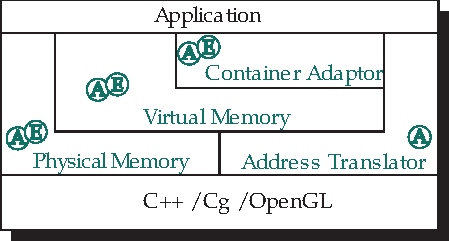
\includegraphics[width=\linewidth]{img/glift-components}
\end{frame}

\begin{frame}
  \frametitle{Virtual memory → Address translator → Physical memory}
  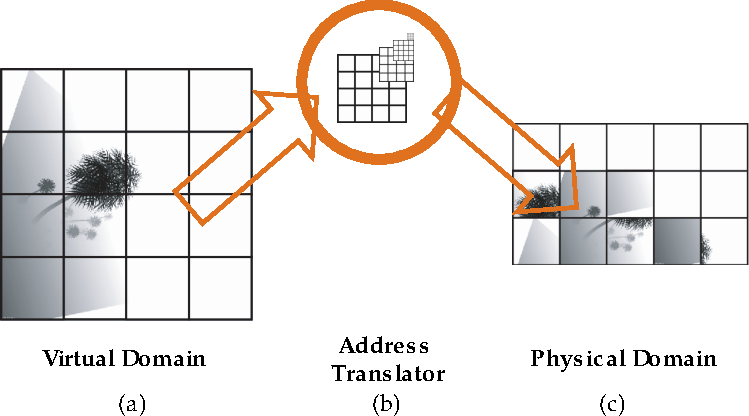
\includegraphics[width=\linewidth]{img/addr-translator}
\end{frame}

\begin{frame}
  \frametitle{Iterators}

  The last component of Glift is iterators. Based on C++'s iterator, they
  designed GPU iterators for parallel work. There are two types of iterators:
  \begin{itemize}
  \item<2-> Element Iterators -- for iterating over the elements in the
    structure
  \item<3-> Address Iterators -- enables address translators to specify
    iteration without having knowledge of physical data
  \end{itemize}
\end{frame}

\begin{frame}[fragile]
  \frametitle{Iterators -- example}
  \begin{ccode*}{gobble=4}
    #include <gliftCg.h>

    float4 main( NeighborIter it ) : COLOR
    {
      // Finite difference discrete Laplacian
      float4 offset( 1, 0, 0, 0 );
      float4 laplace = -8 * it.value( 0 );
      for ( float i = 0; i < 4; ++i ) {
        laplace += it.value( offset );
        laplace += it.value( -offset );
        offset = offset.yzwx;
      }
      return laplace;
    }
  \end{ccode*}
\end{frame}

\section{Classification of GPU data structures}
\begin{frame}
  \frametitle{Classification of GPU data structures}

  The authors classify different data structures in terms of Glift concepts.
  \begin{itemize}
  \item<2-> ND-to-MD translators -- done analytically
  \item<3-> Page Table translators -- using the page tables on the GPU
  \item<4-> GPU tree structures -- $k$-d trees, quadtrees, octrees\ldots
  \item<5-> Dynamic GPU structures -- usually adaptive and sparse
  \end{itemize}
  \onslide<6->{Usually easy to create different structures with Glift, but some
    are challenging to port.}
\end{frame}

\section{Case Studies}
\begin{frame}[fragile]
  \frametitle{Case Studies}

  \only<1,3->{\vspace{15mm}
    We've already seen one! \vspace{3mm}

    \uncover<3->{Also describes a GPU stack. While simple, is useful for e.g.
      $k$-d tree traversal.\vspace{3mm}}

    \uncover<4->{Covers the implementation details of dynamic multiresolution
      adaptive data structures for real time usage, and implements adaptive
      shadow maps as a case.}}
  \begin{overprint}
    \vspace{-5mm}
    \onslide<2>
    \begin{ccode*}{gobble=6}
      #include <gliftCg.h>

      float4 main( NeighborIter it ) : COLOR
      {
        // Finite difference discrete Laplacian
        float4 offset( 1, 0, 0, 0 );
        float4 laplace = -8 * it.value( 0 );
        for ( float i = 0; i < 4; ++i ) {
          laplace += it.value( offset );
          laplace += it.value( -offset );
          offset = offset.yzwx;
        }
        return laplace;
      }
    \end{ccode*}
  \end{overprint}
\end{frame}

\end{document}
